% Drawing 154/03-7 -- folder 154, batch 03, archive page 52 (PDF page 53).
% Transcription: page de dessins, sans texte de sa main : sur la moitié inférieure droite, deux figures séparées par un grand arc rouge. Chacune montre des faisceaux de droites rouges concourant en un point, et une ligne brisée verte (le bord d'une face) qui serpente entre elles, portant des sommets marqués de points noirs ou orangés ; dans la figure de gauche, un segment vert foncé relie le point de concours à un sommet, et une corde verte en pointillé longe le bas ; dans celle de droite, une corde verte en pointillé, jalonnée de points rouges, passe par le point de concours (point rouge épais). Ce sont vraisemblablement des illustrations du bord $\partial F$ et de ses sommets critiques, pages 49 à 51
% Kind: pencils of red lines with a green face boundary (two figures). Method 2 (schematic redraw from the facsimile). Status: partial.
% Notes: Lower right half of a printed listing sheet (CRAY2 job banner, 16 Aug 82, and a typed notice of the computing centre; not reproduced): two figures separated by a large red arc. Each shows a pencil of red lines concurrent at a point and a green broken line (the boundary of a face) winding between them, with vertices marked by black or orange points; on the left a dark green segment joins the point of concurrence to a vertex and a green dotted chord runs along the bottom; on the right a green dotted chord with red points passes through the point of concurrence (thick red point). Read from the page view; the rays and the broken lines are approximate. Still differs from the facsimile: Lower right half of a printed listing sheet (CRAY2 job banner, 16 Aug 82, and a typed notice of the computing centre; not reproduced): two figures separated by a large red arc. Read from the page view; the rays and the broken lines are approximate.
% Coordinates: 1 unit = 1 mm = 1/100 of the crop width (bbox in page fractions: [0.474, 0.332, 0.937, 0.518]).
% Redrawn by Claude (claude-opus-5-5), issue #73, 2026-11-07; not checked by a human; not compiled (no TeX in the session).
% Revised by Claude (claude-opus-5-5) 2026-11-09 (issue #128) after Michel's check: vertices snapped to exact intersections (drawn points on their lines, meeting ends on the stroke they meet, near-concurrent lines through one computed point, curve ends on their rim); labels at \small as in folder 80 batch 3. Status: partial.
% Rights: reproduces part of the work -- behind RENDER_TRANSCRIPTS, never published by itself.
\documentclass[tikz,border=3pt]{standalone}
\usepackage{amsmath,amssymb}
\usetikzlibrary{patterns,arrows.meta}
\tikzset{Or/.style={orange!90!black}, Ye/.style={yellow!80!orange}, Lg/.style={green!60!black!70}, Dg/.style={green!45!black}, Br/.style={brown!80!black}, Rd/.style={red!85!black}, Bl/.style={blue!70!black}, Gy/.style={black!40}, pencil/.style={black!45}, struck/.style={black!35}, mark/.style={circle,draw,inner sep=1.3pt}, pt/.style={circle,fill,inner sep=0.9pt}, opt/.style={circle,draw,fill=white,inner sep=1.1pt}}
\begin{document}
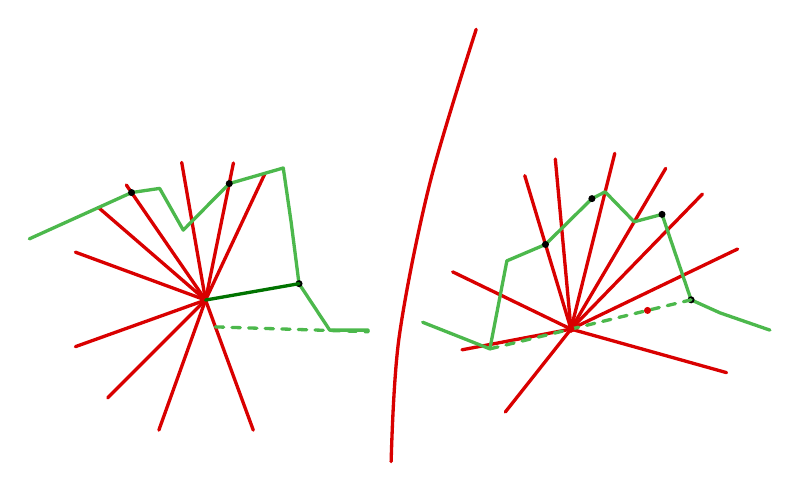
\begin{tikzpicture}[x=1mm,y=1mm,line cap=round,line join=round,font=\scriptsize]
\draw[Rd,very thick] plot[smooth, tension=0.55] coordinates {(58.8,-1) (52.9,-20.6) (49,-40.2) (48,-55.9)};
\draw[Rd,very thick] (24.43,-35.38) -- (31.99,-19.28);
\draw[Rd,very thick] (24.43,-35.38) -- (27.97,-17.97);
\draw[Rd,very thick] (24.43,-35.38) -- (21.4,-17.9);
\draw[Rd,very thick] (24.43,-35.38) -- (14.37,-20.77);
\draw[Rd,very thick] (24.43,-35.38) -- (10.83,-23.63);
\draw[Rd,very thick] (24.43,-35.38) -- (7.9,-29.3);
\draw[Rd,very thick] (24.43,-35.38) -- (7.9,-41.3);
\draw[Rd,very thick] (24.43,-35.38) -- (12,-47.8);
\draw[Rd,very thick] (24.43,-35.38) -- (18.5,-51.9);
\draw[Rd,very thick] (24.43,-35.38) -- (30.49,-51.9);
\draw[Lg,very thick] (2.05,-27.61) -- (15.03,-21.73) -- (18.6,-21.2) -- (21.6,-26.5) -- (27.44,-20.59) -- (34.3,-18.61) -- (35.3,-25.5) -- (36.3,-33.3) -- (40.2,-39.2) -- (45.1,-39.2);
\node[pt] at (15.03,-21.73) {};
\node[pt] at (27.44,-20.59) {};
\node[pt] at (36.3,-33.3) {};
\draw[Dg,very thick] (24.43,-35.38) -- (36.3,-33.3);
\draw[Lg,dashed,very thick] (25.68,-38.79) -- (45.1,-39.4);
\draw[Rd,very thick] (70.84,-39.07) -- (92,-28.9);
\draw[Rd,very thick] (70.84,-39.07) -- (87.53,-21.92);
\draw[Rd,very thick] (70.84,-39.07) -- (82.87,-18.66);
\draw[Rd,very thick] (70.84,-39.07) -- (76.4,-16.75);
\draw[Rd,very thick] (70.84,-39.07) -- (68.85,-17.47);
\draw[Rd,very thick] (70.84,-39.07) -- (64.97,-19.58);
\draw[Rd,very thick] (70.84,-39.07) -- (55.81,-31.8);
\draw[Rd,very thick] (70.84,-39.07) -- (57,-41.7);
\draw[Rd,very thick] (70.84,-39.07) -- (62.5,-49.6);
\draw[Rd,very thick] (70.84,-39.07) -- (90.6,-44.6);
\node[pt,Rd] at (70.84,-39.07) {};
\draw[Lg,very thick] (52,-38.2) -- (60.54,-41.58) -- (62.7,-30.4) -- (67.6,-28.32) -- (73.5,-22.5) -- (75.18,-21.64) -- (78.87,-25.44) -- (82.4,-24.5) -- (86.09,-35.35) -- (89.77,-37.01) -- (96.1,-39.2);
\node[pt] at (67.6,-28.32) {};
\node[pt] at (73.5,-22.5) {};
\node[pt] at (82.4,-24.5) {};
\node[pt] at (86.09,-35.35) {};
\draw[Lg,dashed,very thick] (60.54,-41.58) -- (86.09,-35.35);
\node[pt,Rd] at (70.84,-39.07) {};
\node[pt,Rd] at (80.56,-36.7) {};
\end{tikzpicture}
\end{document}
